\documentclass[twocolumn]{article}

\usepackage{amsmath,amsbsy}
\usepackage{graphicx}
\usepackage{natbib}
\bibliographystyle{mnras}

\def\eqref#1{Eq.~(\ref{eq:#1})}

\def\vec#1{\ensuremath{\boldsymbol{#1}}}
\def\tr#1{\ensuremath{{#1}^\text{\textsc{t}}}}
\def\expect#1{\ensuremath{ {<#1>} }}
\def\ppp#1{#1^\star}

\def\norm{_\tau}
\def\meas{_\nu}
\def\mean#1{\overline{#1}}

\let\outer=\otimes
\let\hadam=\odot
\def\system#1#2#3{\ensuremath{#1 \pm\ #2\ (\pm #3)}}
\def\raw{\ensuremath{\nu}}
\def\vraw{\ensuremath{\vec\raw}}
\def\rawmean{\ensuremath{\mean\raw}}
\def\vrawmean{\ensuremath{\mean\vraw}}

\def\cot{\ensuremath{\tau}}
\def\vcot{\ensuremath{\vec\cot}}
\def\cotmean{\ensuremath{\mean\cot}}
\def\vcotmean{\ensuremath{\mean\vcot}}

\def\data{\ensuremath{{\scriptstyle V}}}
\def\vdata{\ensuremath{\vec\data}}
\def\datamean{\ensuremath{\mean\data}}
\def\vdatamean{\ensuremath{\mean\vdata}}

\def\mod{\ensuremath{\mu}}
\def\vmod{\ensuremath{\vec\mu}}
\def\error{\ensuremath{\eta}}
\def\verror{\ensuremath{\vec\error}}
\def\relerror{\ensuremath{\error\norm}}
\def\abserror{\ensuremath{\error\meas}}
\def\vrelerror{\ensuremath{\vec\relerror}}
\def\vabserror{\ensuremath{\vec\abserror}}
\def\dev{\ensuremath{\sigma}}
\def\devmean{\ensuremath{\mean\dev}}
\def\reldev{\ensuremath{\dev\norm}}
\def\absdev{\ensuremath{\dev\meas}}
\def\cov{\ensuremath{\Sigma}}
\def\vcov{\ensuremath{\vec\cov}}
\def\abscov{\ensuremath{\cov\meas}}
\def\relcov{\ensuremath{\cov\norm}}
\def\vabscov{\ensuremath{\vec\abscov}}
\def\vrelcov{\ensuremath{\vec\relcov}}
\def\corr{\ensuremath{\varrho}}
\def\sens{\ensuremath{x}}
\def\vsens{\ensuremath{\vec\sens}}
\def\msens{\ensuremath{\vec X}}
\def\param{\ensuremath{p}}
\def\vparam{\ensuremath{\vec\param}}
\def\dataflat{\ensuremath{\mod_0}}
\def\vdataflat{\ensuremath{\vec\dataflat}}
\def\paramflat{\ensuremath{\param\meas}}
\def\vparamflat{\ensuremath{\vec\paramflat}}
\def\paramppp{\ppp{\param}}
\def\vparamppp{\ensuremath{\vec\paramppp}}
\def\datappp{\ppp{\mod}}
\def\vdatappp{\ensuremath{\vec\datappp}}
\def\datarec#1{\mod_{#1}}
\def\vdatarec#1{\ensuremath{\vec\mod_{#1}}}


\begin{document}

\title{Fitting correlated interferometric data}
\author{R\'egis Lachaume}
\maketitle

\begin{abstract}
We show how Peelle's pertinent puzzle can be avoided in the framework of the least squares minimisation.
\end{abstract}

\section{Introduction}

Some widely used long-baseline interferometric observables, like the visibility amplitudes, are usually obtained by normalisation: A set of fringe contrasts obtained on a science target are divided by the intrumental transfer function determined on calibrator stars. The uncertainty in the transfer function results in correlations in the visibilities, as \citet{PER03} thoroughly examined.  In the context of experimental nuclear physics, \citet{PEE87} noted that such correlated measurements could provide an estimate falling below the individual data points, a paradox known as Peelle's Pertinent Puzzle (PPP). 

In this introduction, we rewrite and adapt the original example in the context of long-baseline interferometry. Let's assume the inverse of the instrumental fringe contrast $\cot \pm \cot\reldev$ has been interpolated from one or several calibrator observations. A visibility amplitude is now now estimated from two contrast measurements $\raw_1 \pm \absdev$ and $\raw_2 \pm \absdev$.  For each measurement, visibility amplitudes are:

\begin{subequations}
\begin{align}
    \data_1 &= \system{\cot\raw_1}{\cot\absdev}{\cot\raw_1\reldev},\\
    \data_2 &= \system{\cot\raw_2}{\cot\absdev}{\cot\raw_2\reldev}.
\end{align}
\label{eq:data12}
\end{subequations}

They are normalised with the same quantity (\cot), so they are correlated, hence the systematic uncertainty term between parentheses in \eqref{data12}. Error propagation gives the covariance matrix

\begin{equation} 
   \vcov = \begin{pmatrix} 
     \absdev^2\cot^2 + \reldev^2\data_1^2 & \reldev^2\data_1\data_2\\
     \reldev^2\data_1\data_2              & \absdev^2\cot^2 + \reldev^2\data_2^2
            \end{pmatrix},
\end{equation}
when the second-order error term ($\absdev\reldev$) is ignored.  Using the matrix inverse $\vcov^{-1}$, the least squares estimate is 
\begin{equation}
\begin{split}
    {\data} &= \frac{  (\vcov^{-1}_{11} + \vcov^{-1}_{12}) \data_1
                      +(\vcov^{-1}_{22} + \vcov^{-1}_{12}) \data_2 }
                    {   (\vcov^{-1}_{11} + \vcov^{-1}_{12}) \hphantom{\data_1}
                      + (\vcov^{-1}_{22} + \vcov^{-1}_{12}) \hphantom{\data_2} 
                    },\\
            &= \frac{\data_1 + \data_2}{2} 
            \left(1 + \reldev^2\frac{(\data_1-\data_2)^2}{2\tau^2\absdev^2}\right)^{-1}.
\end{split}
\end{equation}
It systematically falls below the average of the two values $\data_1$ and $\data_2$.  If measurements differ significantly, it can even fall below the lowest value.  Figure~\ref{fig:peelle} gives such an example with a instrumental visibility of 50\% and two measurements on an unresolved target: 
\begin{align*}
    \cot   &= 2.000 \pm 0.100\ (5\%),\\
    \raw_1 &= 0.495 \pm 0.003\ (\approx 0.6\%),\\
    \raw_2 &= 0.505 \pm 0.003\ (\approx 0.6\%),
\intertext{which yields two points 2.4 standard deviations appart}
    \data_1 &= \system{0.990}{0.006}{0.050},\\
    \data_2 &= \system{1.010}{0.006}{0.050}
\intertext{and the estimate}
    \data &= \system{0.986}{0.004}{0.049}
\end{align*}
falls outside the data range.
\begin{figure}[t]
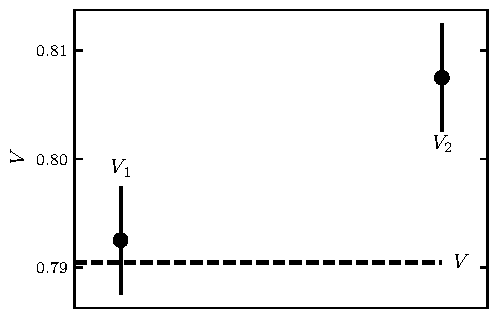
\includegraphics[width=\linewidth]{pdf/original-peelle.pdf}
\caption{Original Peelle problem rewritten in the context of interferometry.  \emph{Bottom:} Two raw visibility amplitudes $\nu_1$ and $\nu_2$ (points with statistic error bars of $\approx 0.6\%$) are calibrated by the transfer function $1/\tau$ (solid line with systematic error zone of 5\%). \emph{Top:} the two calibrated visibility measurements $\data_1$ and $\data_2$ (points with statistic error bars of $\approx 0.6\%$) are strongly correlated. The least-squares estimate for the visibility $\data$ (dashed line, with statistic uncertainty error zone displayed) falls outside of the data range.}
\label{fig:peelle}
\end{figure}

See \cite{PEE87,DAG94,BUR11,NEU12,NEU13,NEU14,NIS14}.


\begin{table}[t]
\caption{Symbols used in this paper. Lower case bold font is used for vectors and upper case bold font for matrices.}
\begin{tabular}{ll}
\hline\hline
Symbol               & Meaning\\
\hline
$\mean a$            & true value of $a$\\
$<a>$                & expectancy of $a$\\
$\tr{\vec A}$        & transpose of $\vec A$\\
$\vec c = \vec a\hadam\vec b$ & elementwise product of $\vec a$ and $\vec b$\\
$\vec C = \vec a\outer\vec b$ & outer product of $\vec a$ and $\vec b$\\
$\vec c = \vec A\vec b$       & matrix product of $\vec A$ and $\vec b$\\
$\delta$             & Kronecker delta\\
\hline
$\vdata$             & data\\ 
$\verror$            & error ($= \vdata - \vdatamean$)\\
$\dev^2$             & variance ($= \expect{\error^2}$)\\
$\vcov$              & covariance matrix ($= \expect{\verror\outer\verror}$)\\
$\corr$              & correlation coefficient\\
$\vsens$, $\msens$   & sensitivity vector or matrix\\
$\vparam$            & parameters of the model\\
$\vmod$              & model values ($= \vsens\vparam\approx\vdatamean$)\\
\hline
$a\meas$             & $a$ of the measurement error\\
$a\norm$             & $a$ of the normalisation error\\
$\ppp a$             & $a$ impacted by PPP\\
\hline
\end{tabular}
\end{table}

\section{Single value fit}

We consider a set of measurements of a single normalised quantity, like the visibility amplitude, given by a vector $\vdata = \tr{(\data_1, \cdots, \data_n)}$. It is derived from an uncalibrated quantity like the fringe contrast, $\vraw = \tr{(\raw_1, \cdots, \raw_n)}$ and a normalisation factor, like the cotransfer function, $\vcot = \tr{(\cot_1, \cdots, \cot_n)}$ by 
\begin{equation}
    \vdata = \vcot\hadam\vraw,
\end{equation}
where $\hadam$ denotes the Hadamard (elementwise) product of vectors. We note $\datamean$, $\cotmean$, and $\rawmean$ the true, but unknown, values of these quantities.  The error vector on $\vdata$  
\begin{align}
    \verror    &= \vdata - \datamean, \\
\intertext{can be written as a sum of measurement and normalisation errors if we ignore a second-order term:}
    \verror    &= \vabserror + \datamean \vrelerror.\\
\intertext{These errors are given by}
    \vabserror &= \cotmean (\vraw - \rawmean), \\
    \vrelerror &= \frac1\cotmean (\vcot-\cotmean).
\end{align}

We assume $\vabserror$ and $\vrelerror$ are independent error terms of mean 0 and standard deviations are $\absdev$ and $\reldev$, respectively. In addition, we consider correlation of the normalisation errors, with correlation coefficient $\corr$.  In the case of interferometry, it can arise from the uncertainty on the calibrators' geometry.  The covariance matrix is given by
\begin{align}
    \vcov     &= \expect{\verror\outer\verror},\\
\intertext{where $\outer$ denotes the outer product of vectors and $\expect{}$ stands for the expectancy, so that}
    \cov_{ij} &= \left[ \absdev^2 
                  + (1-\corr)\reldev^2\datamean^2
                \right] \delta_{ij} 
            + \corr\reldev^2\datamean^2.
\end{align}

The value $\datamean$ is yet to be determined, so the covariances are often derived using the data in the propagation:
\begin{equation}
    \ppp{\cov_{ij}} = \left[ 
                    \absdev^2 
                  + (1-\corr)\reldev^2 \data_i^2
                \right] \delta_{ij} 
            + \corr\reldev^2\data_i\data_j. \label{eq:cov}
\end{equation}

The least squares estimate for $\datamean$ is given by
\begin{equation}
    \ppp{\mod} =
                  \frac { \tr\vsens{\ppp\vcov}^{-1}\vdata }
                        { \tr\vsens{\ppp\vcov}^{-1}\vsens }
\end{equation}
where $\vsens = \tr{(1, \cdots, 1)}$ is the trivial sensitivity vector.  The covariance matrix is the sum of an invertible diagonal matrix and one of rank one (see \eqref{cov}), so that the inverse is obtained using the Woodbury matrix identity: 
\begin{align}
    \{ {\ppp\vcov}^{-1} \}_{ij} &= \frac{\delta_{ij}}{\dev_i^2}
         - \frac{\corr\reldev^2\data_i\data_j}
                {\dev_i^2\dev_j^2\Big(1 + 
            \corr\reldev^2\sum\limits_{k} \frac{\data_k^2}{\dev_k^2}\Big)},\\
  \intertext{where}
  \dev_i^2 &= \absdev^2+(1-\corr)\reldev^2\data_i^2.
\end{align}
It allows us to put the least squares estimate in the relatively compact form 
\begin{equation}
  \ppp{\mod} = 
    \frac { 
      \sum\limits_i \frac{\data_i}{\dev_i^2}
    }{ 
      \sum\limits_i 
          \Big( 1   
             + \corr\reldev^2\sum\limits_{j} \frac{(\data_i-\data_j)^2}{\dev_j^2}
           \Big)
          \frac{1}{\dev_i^2} 
   }.\label{eq:mu}
\end{equation}


For small enough errors ($\error_i \ll \datamean$) the second-order Taylor development in $\error_i = \data_i - \datamean$ yields 
\begin{equation}
    \ppp{\mod} \approx  \datamean 
                  +\frac1n {\sum\limits_i \error_i}
                       - \frac {[2 + (n - 2)\corr]\reldev^2\datamean^2
                          }{
                           2n^2 \devmean^2             
                          }
                           \sum\limits_{i\ne j} (\error_i-\error_j)^2
\end{equation}
where
\begin{equation}
    \devmean^2 = \absdev^2+(1-\corr)\reldev^2\datamean^2 
\end{equation}

Since $\expect{\error_i} = 0$ and $\expect{(\error_i-\error_j)^2} = 2\devmean^2$, the expectancy
\begin{equation}
    \expect{\ppp{\mod}} \approx \datamean 
            \left[ 1 -  
             \left(1-\frac1n\right)
             \left(2 + (n-2)\corr\right)
              \reldev^2 \right]
\end{equation}
is biased.  If the data are not correlated ($\corr = 0$), the bias is small
($\reldev^2$ to $2\reldev^2$) but it becomes large for correlated data if the number of points is large ($\sim n\reldev^2$ for fully correlated data).
Figure~\ref{fig:uncorr-peelle} shows a simulation of the bias as a function of
the normalisation uncertainty $\reldev$ for various data sizes ($n = 2$ to
100). 
\begin{figure}[t]
\centering
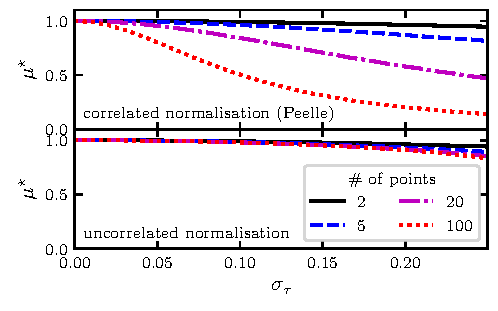
\includegraphics[width=\linewidth]{pdf/uncorrelated-peelle.pdf}
\caption{Fit $\datappp$  to unresolved visibilities ($\data = 1$), as a function of the relative uncertainty on the calibration $\reldev$ and the number of measurements $n$. $2/n\times10^5$ simulations were made and averaged, assuming that $\abserror$ and $\relerror$ follow normal distributions. \textit{Top:} fully correlated normalisation like in original Peelle's puzzle ($\absdev=0.02$ and $\corr = 1$). \textit{Bottom:} normalisation error without correlation ($\absdev=0.02$ and $\corr = 0$).}
\label{fig:uncorr-peelle}
\end{figure}

\section{Model fitting}
We now consider a set of measurements corresponding to the linear model 
\begin{align}
    \vmod  &= \msens\vparam,\\
\intertext{where $\vparam$ are the unknown parameters and $\msens$ is the known sensitivity matrix. Typically, $\sens_{ik}=f_k(u_i, v_i)$ for a linear model and $\sens_{ik} = \partial f/\partial p_k(u_i, v_i)$ for a non-linear model that we choose to approximate by a linear one close to a solution. $(u, v)$ is the reduced baseline.  The true values $\vdatamean$ are are impacted by errors so that the data are} 
    \vdata &= \vdatamean + \verror\\
\intertext{with the error term $\verror$ again expressed as the sum of a measurement error and a normalisation one:}
    \verror &=  \vabserror + \vrelerror \hadam \vdatamean.
\end{align}
The measurement errors $\vec\abserror$ and normalisation errors $\vec\relerror$ following multivariate distributions of mean zero and covariance matrices $\vabscov$ and $\vrelcov$ respectively. Given the covariance matrix $\vcov$ of this model, the least squares estimate is
\begin{align}
   \vparam &= (\tr\msens \vcov^{-1} \msens)^{-1} (\tr\msens \vcov^{-1} \vdata)
\end{align}
We investigate four ways to determine the covariance matrix
\begin{enumerate}
    \item Ignoring the correlations in the normalisation using $\vcov_0 = \vabscov + (\vdata\outer\vdata)\hadam(\vrelcov\hadam\vec I)$. We note $\vdataflat = \msens(\tr\msens\vcov_0^{-1}\msens)^{-1}\tr\msens\vcov_0^{-1}\vdata$ the resulting model of the data. 
    \item Using the na\"\i{}ve estimate $\ppp\vcov = \vabscov + (\vdata\outer\vdata)\hadam\vrelcov$ which is known to lead to Peelle's pertinent puzzle in the trivial case of a constant model. 
    \item Using the data model of the fit without the normalisation error: $\vcov_1 = \vabscov + (\vdataflat\outer\vdataflat)\hadam\vrelcov$.  The resulting least squares model is $\vdatarec{1} = \msens(\tr\msens\vcov_1^{-1}\msens)^{-1}\tr\msens\vcov_1^{-1}\vdata$.
    \item Recursively fitting the data by updating the data model in the covariance matrix. We derive $\vdatarec{k} = \msens(\tr\msens\vcov_k^{-1}\msens)^{-1}\tr\msens\vcov_k^{-1}\vdata$ using $\vcov_{k} = \vabscov + (\vdatarec{k-1}\outer\vdatarec{k-1})\hadam\vrelcov$, starting with the estimate $\vdatarec{1}$ ($k = 2$). 
\end{enumerate}

Figure~\ref{fig:fitexample} shows the example of a quadratic fit to partially correlated data with the four methods above.  As expected, the use of data $\vdata$ in the correlation matrix (method 2) leads to grossly underestimated data values, in the very same way as in the classical Peelle case (constant model).  Both method 3 and 4 yield reasonable estimates.

\begin{figure}[t]
\centering
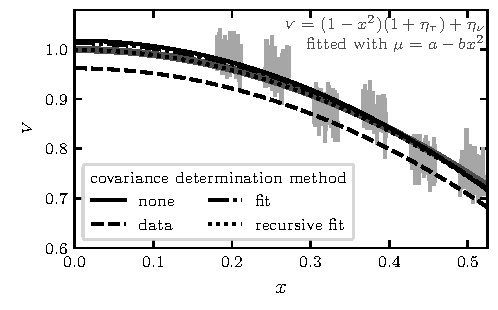
\includegraphics[width=\linewidth]{pdf/fit-example.pdf}
\caption{Example of a fit of correlated data from a four telescope interferometer with medium resolution: 6 groups of 100 data points (light gray points with the measurement error bar) with 2\% uncorrelated measurement errors and 3\% correlated normalisation error follow model $1-u^2$ (thick gray line). Least-squares model fitting of $a-bu^2$ is performed using four prescriptions for the covariance matrix.}
\label{fig:fitexample}
\end{figure}

\begin{figure*}[t]
\centering
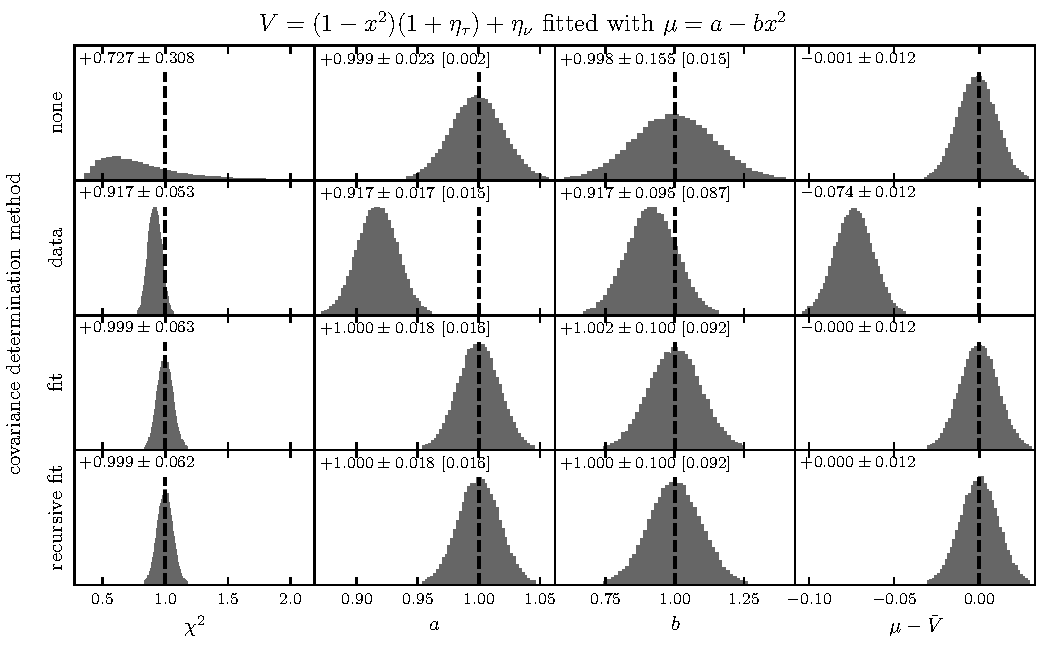
\includegraphics[width=\linewidth]{pdf/fit-quality.pdf}
\caption{Distribution of the fitted parameters and fit properties for the four covariance matrix prescriptions. $5\times10^4$ simulations of 6 groups of 100 correlated data points $\data$ ($\absdev = 2\%$, $\reldev = 3\%$, $\corr = 1$, normal distributions) following model $\mod = 1-u^2$ are performed and fitted with $a - bu^2$ using least-squares minimisation. These groups of points are typical of a single snapshot obtained with a four-telescopes interferometer with medium spectral resolution. Reported quantities include median and 1-$\sigma$ interval of their distribution and, within brackets, the median uncertainty reported by the least squares fit: \emph{leftmost column:} distribution of the least squares; \emph{middle left:} constant coefficient $a$; \emph{middle right:} quadadratic coefficient $b$; \emph{rightmost column:} mean difference between model and data. The covariance matrix prescriptions are: \emph{top row:} correlations are ignored; \emph{second row:} a na\"\i{}ve covariance matrix uses the data values; \emph{third row:} covariance matrix uses modelled values from fit without correlations; \emph{bottom row:} covariance matrix and model are recursively computed, with the covariance matrix of the next recursion using the modelled value of the last step.}
\end{figure*}

\section{Conclusion}
\begin{enumerate}
\item Peelle's pertinent puzzle primarily arises from an incorrect description of the relative uncertainties.  It will occur in a fully linear problem and, to some extent, without correlations.
\item For uncorrelated data, the relative bias is of the order of the square of the relative uncertainty as long as errors remain small. It increases twofold when the number of data points becomes large.
\item For correlated data, the relative bias is larger by a factor of the order of the number of correlated points as long as the resulting error remain small.
\item In least-squares model fits, the problem disappears if the uncertainties, or the covariance matrix, are updated with the model values instead of the measurement values.
\end{enumerate}

\bibliography{article}

\end{document}
